% !TeX spellcheck = en_US
% !TeX encoding = UTF-8
\chapter{Data Collection-Subject Study}

A collaborative assembly task involving wooden pieces was designed in the robot laboratory of the Institute of Control Theory and Systems Engineering at the Technical University of Dortmund. This setup aims to accurately replicate tasks commonly seen in industrial settings where collaboration between humans and cobots is frequently observed. The Universal Robot UR10 was selected as the cobot to be used in the study. A call for participants invite was sent out, and 20 male students who all had a technical background volunteered to participate in the study. Seventeen of the students did not have any previous experience working with a robot in any way, whereas the remaining
had some previous experience with robots. The mean age of the participants were $23 \pm 2$ years. Before the experiment began, all participants were given a comprehensive overview of the study's objectives and procedures, along with a consent form. Only those participants who agreed to the terms and signed the consent form were permitted to proceed with the experiment. To ensure the ethical integrity of the study, a prior request for ethical approval was submitted to the appropriate ethics council and permission was obtained to conduct the subject study.

\section{Design of Tasks}
For the purpose of studying the impact of stress on various factors, the assembly of different mock items using wooden children's toys was chosen as a method of replicating an industrial assembly task.

\begin{table}[h]
    \centering
    \renewcommand{\arraystretch}{2}
    %\resizebox{\columnwidth}{!}{%
    \begin{tabular}{|c|c|c|c|}
    \hline
    \textbf{\makecell{Collision Avoidance \\ Strategy}} & \textbf{\makecell{Seperated \\Workspace (A)}} & \textbf{\makecell{Shared \\Workspace (B)}} & \textbf{\makecell{Shared Workspace with \\ Direct Collaboration (C)}} \\ \hline
    \textbf{\makecell{No Collision \\Avoidance (X)}} & AX  & BX  & CX \\ \hline
    \textbf{\makecell{Dynamic Collision \\Avoidance (Y)}}        & Not Required                               & BY                           & CY                                                    \\ \hline
    \textbf{\makecell{Predictive Collision \\Avoidance (Z)}}    & Not Required     & BZ                           & CZ                                                    \\ \hline
    \end{tabular}
    
\caption{Task names for different Collision Avoidance Strategies and Workspace Scenarios}
\label{table:tasks}
\end{table}

These included three distinct levels of different collaboration levels:

\begin{itemize}
    \item \textbf{Seperated Worksapce}:
    Human and cobot have no overlapping workspace. The cobot works in the background.The human already has all items required for the assembly task in front of him.
    
    \item \textbf{Shared Workspace}:
    The human and cobot share the same work area.The cobot brings each item required for the assembly tasks to the human and places it on the table in front of the human.
    
    \item \textbf{Shared Workspace with Direct Collaboration}:
    The human and cobot share the same work area and the cobot brings the item required for the assembly tasks to the human and  directly hands over the items to the human.
\end{itemize}

As well as three robot collision avoidance strategies:

\begin{itemize}
    \item \textbf{No Collision Avoidance}:
    No collision avoidance measures are in place, and the robot stops at a collision.
    
    \item \textbf{Dynamic Collision Avoidance}:
    The robot identifies the human as a dynamic obstacle and adjusts its trajectory to avoid collisions.
    
    \item \textbf{Predictive Collision Avoidance}:
    This strategy uses predictions to predict the human's future position and adjusts its trajectory to avoid collisions.
\end{itemize}

The \autoref{table:tasks} shows the various combinations of factors and the naming conventions of the tasks, yielding seven experimental scenarios since collision avoidance is not applicable when Separated Workspaces are involved. For example, task BZ employed a predictive collision avoidance strategy while doing the task in a shared workspace. So a within-subject experimental design was employed where each participant was tested on all seven scenarios. By having the same participants perform each task, we minimized the impact of differing skill sets, experiences, and cognitive abilities, which could otherwise skew the results.

\begin{figure}[h]
	\centering
	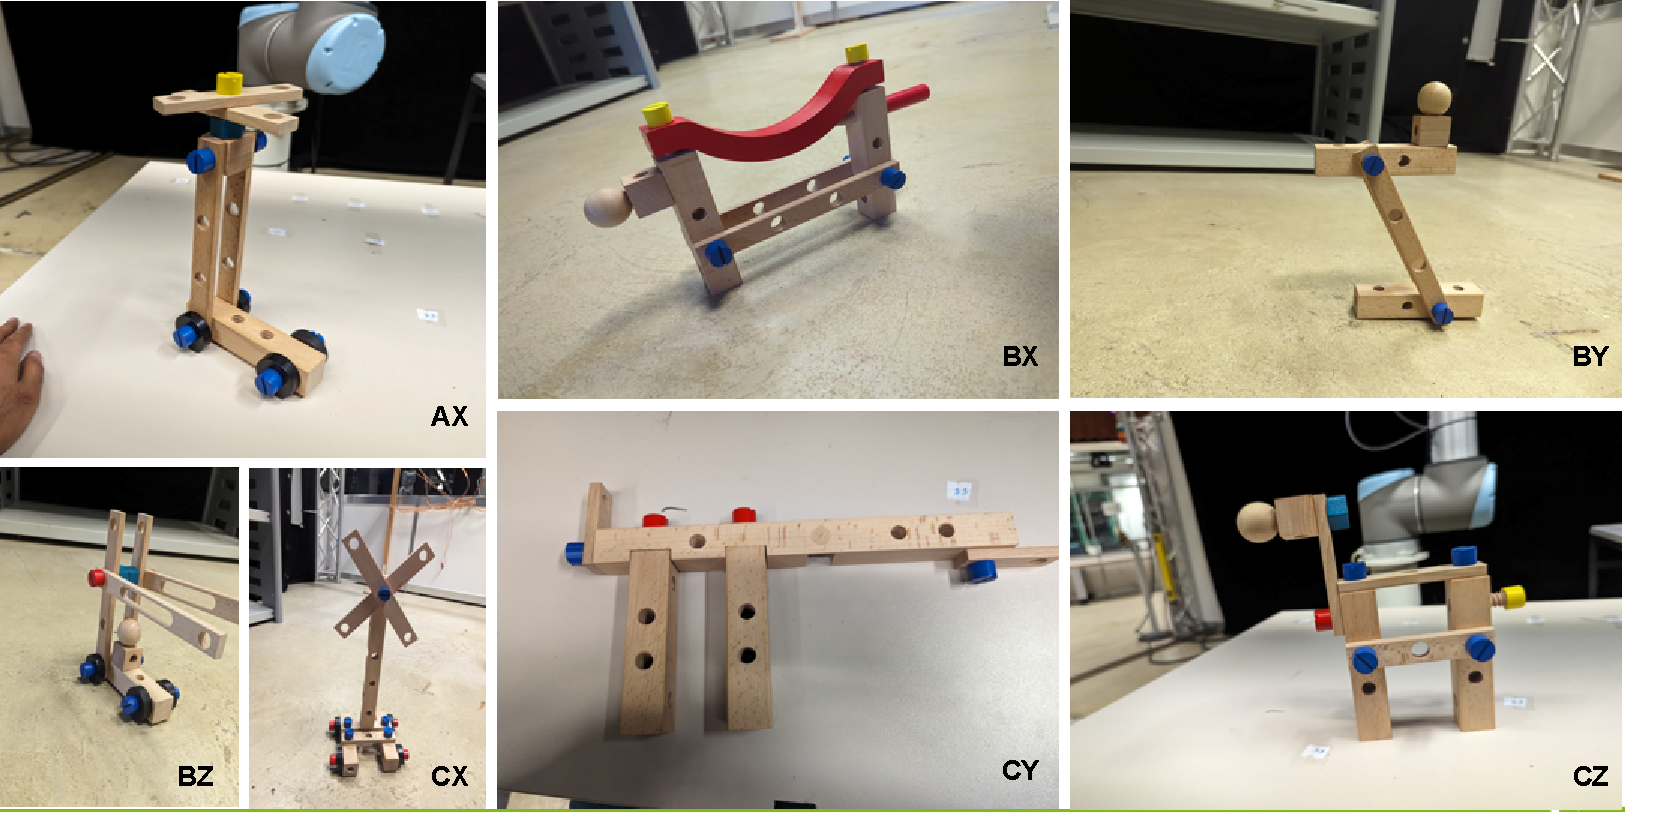
\includegraphics[width=0.8\columnwidth]{images/tasks.drawio.pdf}
	\caption{7 different assembly tasks}
	\label{fig:task}
\end{figure}


To avoid any potential learning effects and ensure that each task measures the intended
variables accurately, we had to design seven different assembly tasks. Each task involved
assembling a unique item, chosen of similar complexity and required effort. This
similarity in task difficulty was crucial to avoid the introduction of other variables, such
as familiarity with the task, which could affect the results.   \autoref{fig:task} shows the final assemblies completed in each of the seven tasks. Each task had approximately 4-6 different
parts, which were supposed to be screwed together to complete the tasks. By standardizing
the complexity across tasks, we aimed to isolate the impact of the collision avoidance
strategies and collaboration levels. We also had to consider the order in which the task
was administered for each participant, ensuring that learning or fatigue does not affect the
outcomes in any way. Each participant experienced the tasks in a unique order, balancing out any potential biases introduced by the order of task presentation.


\section{Apparatus and Experimental Setup} \label{sec:expprot}
The experiment was set up in a specially designated area of our laboratory. \autoref{fig:setup} shows the experimental setup. 
 At the center of this arrangement was the collaborative workspace, featuring a table and chairs for the human participant (Area B in  \autoref{fig:setup}), positioned directly opposite the robot's dedicated workspace. Adjacent to this, on the right side of the collaborative workspace, a table was placed to hold the various items needed for the assembly tasks(Area A \autoref{fig:setup}). The robot would pick the necessary items from this table for each specific task and deliver them to the human participant. In front of the human participant, a mobile device was also placed. This device was key to the experiment, as it presented the participant with concise, step-by-step instructions for each assembly task. \autoref{fig:phone1} shows how these instructions were visually displayed, offering clear and easy-to-follow guidance. The participant would start the assembly task as soon as the first item is delivered to the human participant. The robot would then proceed to the next item, and so on until all items are delivered to the human participant.



 
\begin{figure}[h] 

    \centering 

    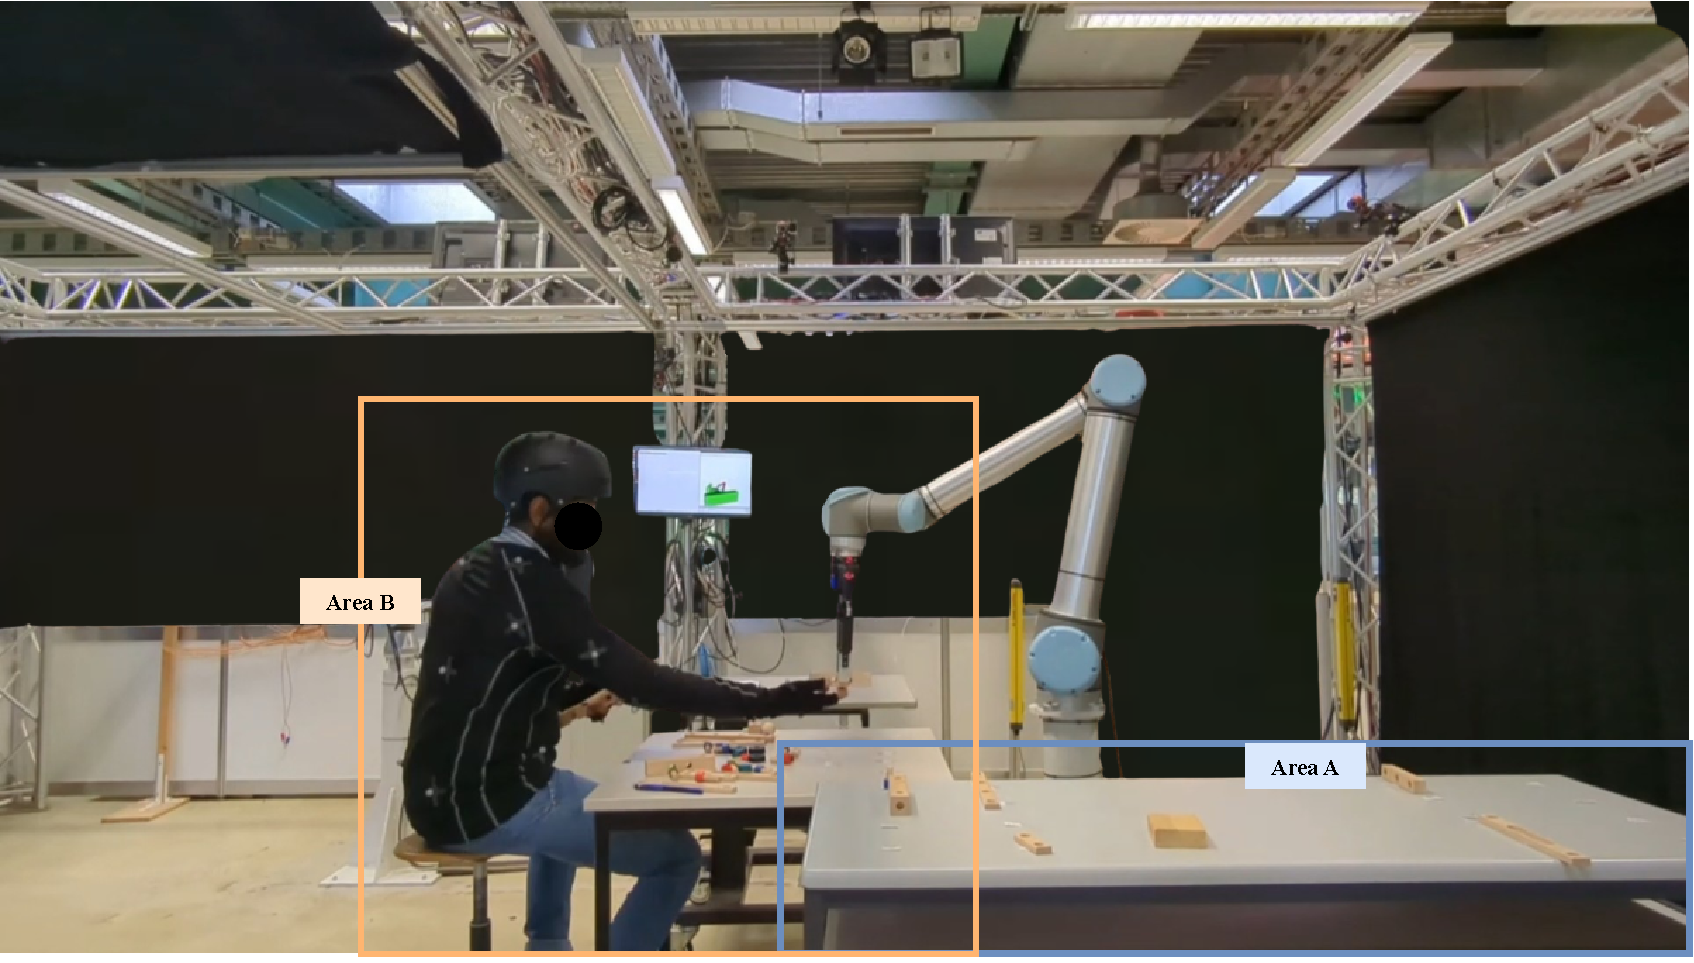
\includegraphics[width=0.7\columnwidth]{images/handover.pdf} 

    \caption{The experimental setup} 

    \label{fig:setup} 

\end{figure} 



The entire experimental area had an OptiTrack motion capture system, outfitted with 12 high-precision cameras fitted across all 4 sides as partly seen in \autoref{fig:apparatus}. These OptiTrack cameras, known for their accuracy and low latency are used to capture every detail of the human participant's movements. This setup was necessary for the collision avoidance trajectory planning for the robot and also providing a detailed and continuous record of the participant's interactions with the robot. The use of the OptiTrack system enabled us to gather precise data on human motion. The participants were equipped with the motion capture suit which had 25 distinct marker points which were used to capture the human's head and upper body. To prioritize participant safety, especially given the proximity to a large robotic arm, a helmet also equipped with the head markers was provided to each participant.

\begin{figure}[hb]
	\centering
	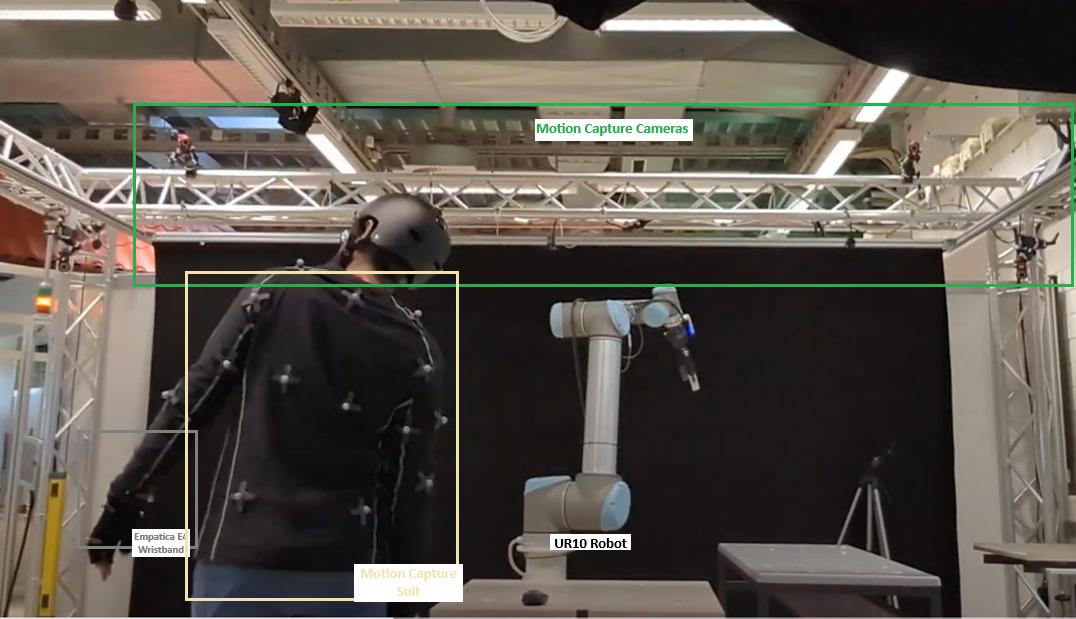
\includegraphics[width=0.8\columnwidth]{images/apparatus.png}
	\caption{Apparatus used}
	\label{fig:apparatus}
\end{figure}

For capturing the physiological signal of the participants, the Empatica E4 wristband was equipped on the participant's non-dominant hand. The participant's physiological signals such as \gls{GSR}, \gls{EDA}, \GLS{HR} and temperature, are captured by the Empatica E4 wristband, which transmits data wirelessly via Bluetooth to a Windows PC. This PC with an Intel i5-12600KF at 3.7 GHz using
32 GB RAM and a NVIDIA GeForce RTX 3060 with 12 GB
VRAM.
runs the E4 streaming server aswell, facilitating the real-time transfer of this data. The various motion capture cameras recording the participant's movements are synced  together and are connected to the Windows PC as well running the motion capture software, Motive.
The physiological data from the Empatica E4 and the motion data from the motion capture system are then streamed to a Linux PC running the Robot Operating System (ROS)1 Melodic.
The motion capture data is published to \textit{/tf} topic. Whereas the Empatica E4 node is available as a ROS2 node running inside a docker container interfacing with the ROS1 using a ROS bridge.
Then a data synchronization script is used to create a ROS node that subscribes to the multiple topics from various sources, synchronizes the incoming data, and publishes a compiled message to the \textit{/aggregated\_data} topic. A more detailed description of the data synchronization process is provided in  \autoref{sec:synchronization}.
This synchronized data topic is then recorded to a rosbag. A general schematic of this is shown in \autoref{fig:netwrok}.


\begin{figure}[h]
	\centering
	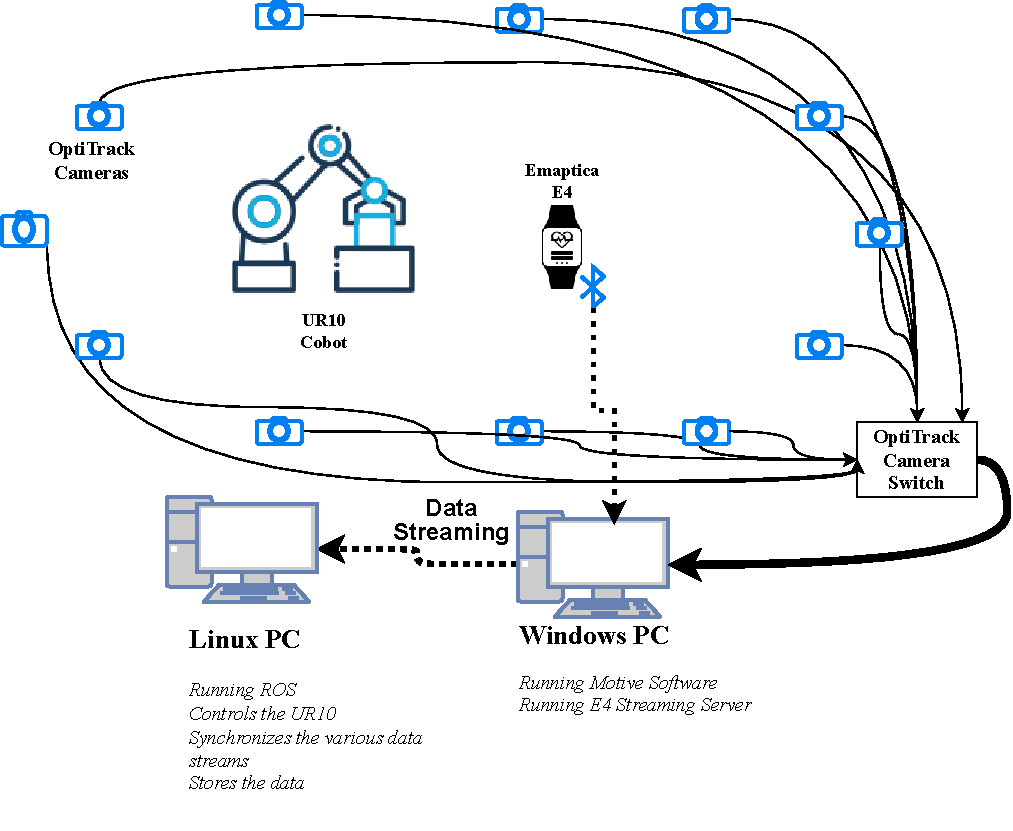
\includegraphics[width=0.9\columnwidth]{images/Experiment system.drawio.pdf}
	\caption{Schematic of the experiment setup}
	\label{fig:netwrok}
\end{figure}


\section{Experimental Procedure}
The participants visited the experiment room in the time slot they had selected. 
Upon arrival, they were greeted and guided through a comprehensive orientation that explained the experimental procedures. This session included detailed descriptions of the various equipment involved, such as the Empatica E4 wristband for monitoring physiological responses and the motion capture system for observing and recording precise movement. Each participant was fitted with the motion capture suit and the Empatica E4 wristband, which was placed on their non-dominant hand, and both were carefully calibrated for accurate data collection.

Participants then were given an initial questionnaire that included a consent form, general information, and questions about their prior experience with cobots as well as the General Attitudes Towards Robots Scale (GAToRS) questionnaire \autocite{gatrs}.

\begin{figure}[h]
    \centering
    % First image
    \begin{subfigure}[b]{0.45\columnwidth}
        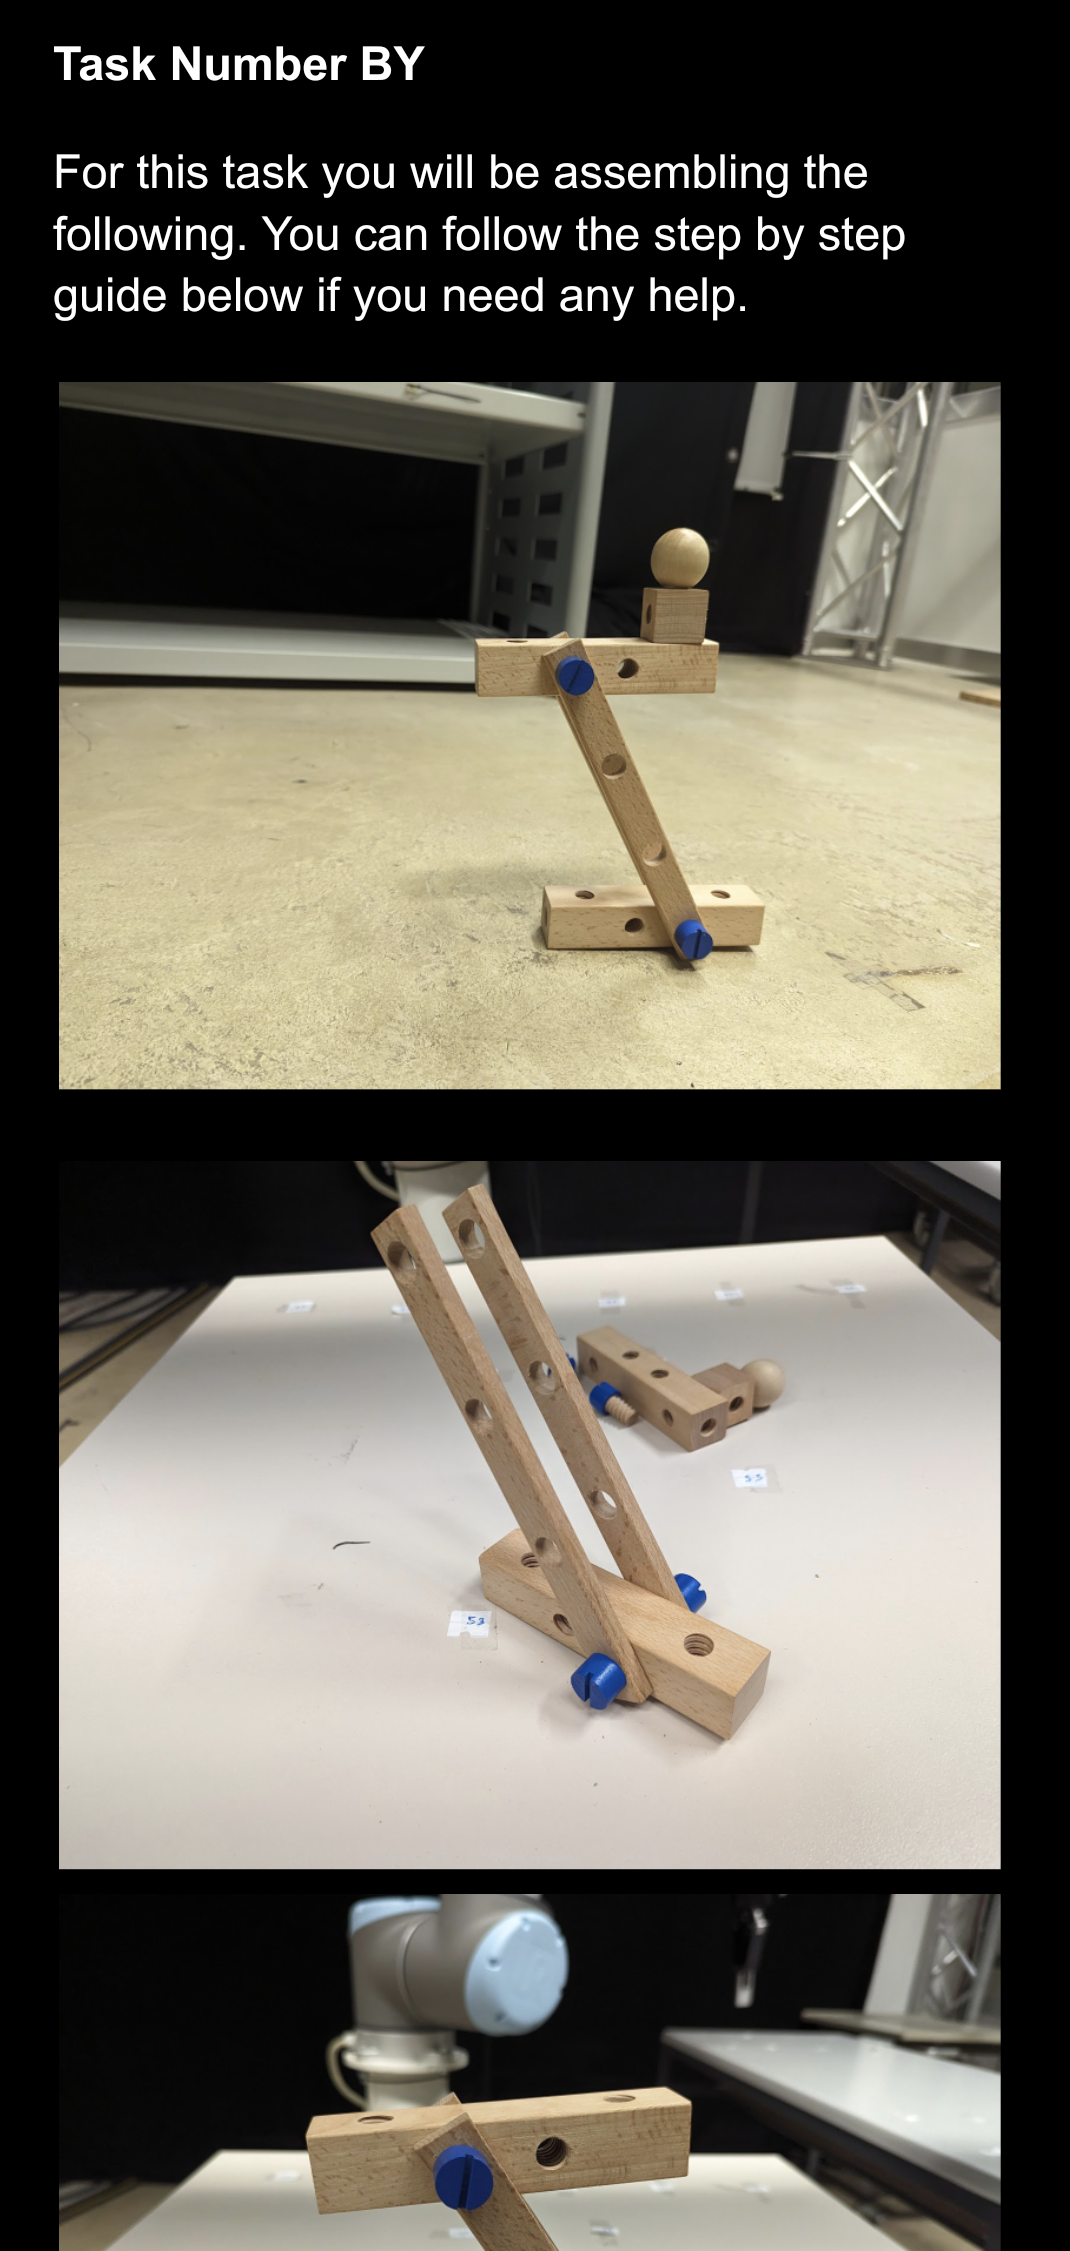
\includegraphics[width=\textwidth]{images/sts.png}
        \caption{Step by Step Task instructions}
        \label{fig:phone1}
    \end{subfigure}
    % Second image
    \begin{subfigure}[b]{0.45\columnwidth}
        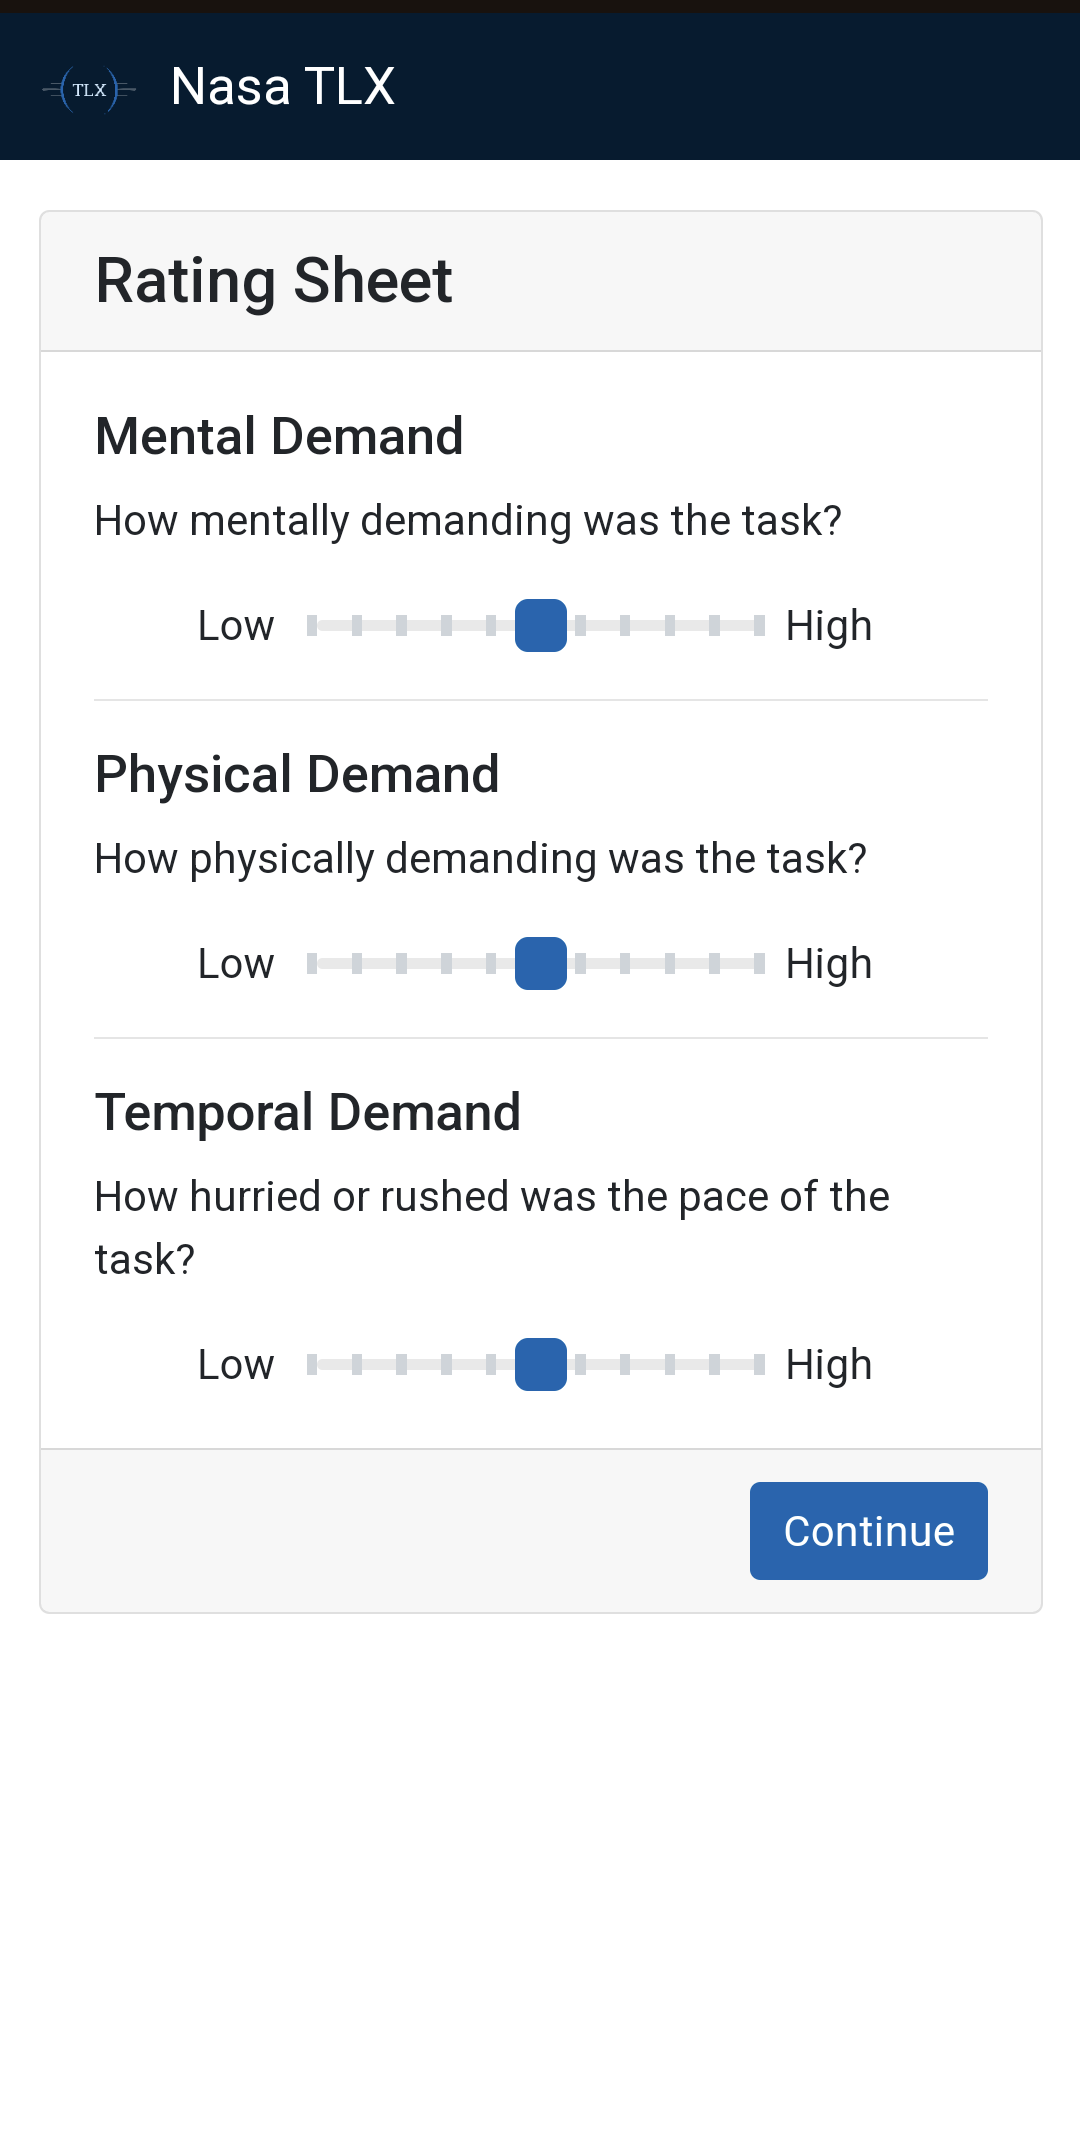
\includegraphics[width=\textwidth]{images/nasa.png}
        \caption{NASA-TLX Questionnaires}
        \label{fig:phone2}
    \end{subfigure}
    \caption{Screenshots from mobile device}
    \label{fig:phone}
\end{figure}

\begin{figure}[h]
	\centering
	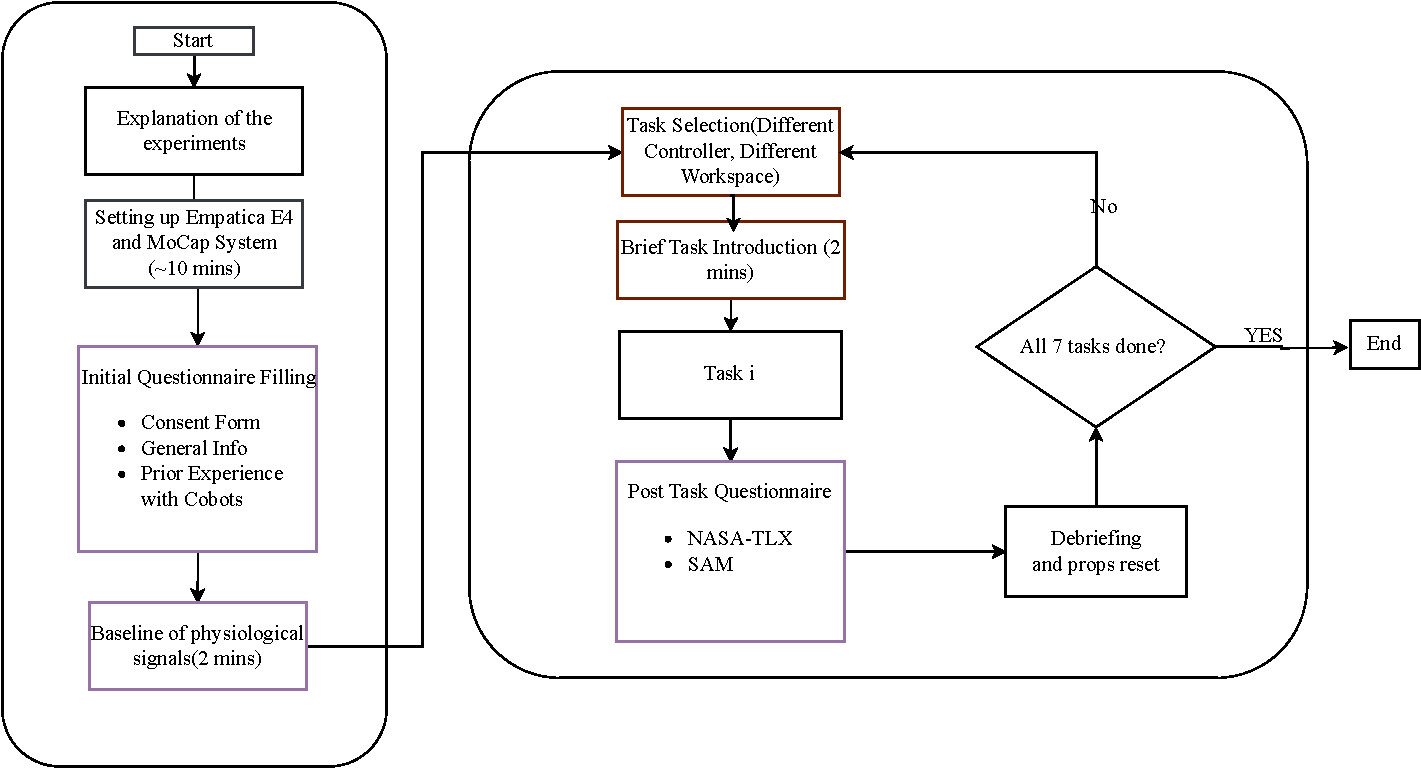
\includegraphics[width=\columnwidth]{images/expschematic.pdf}
	\caption{Schematic of the experiment protocol}
	\label{fig:prot}
\end{figure}

Once the preliminary documentation was complete, we established a baseline of physiological signals for each participant, which involved recording data for 2 minutes without any interaction with the cobot. This step ensured that we had a standard reference point for each participant's physiological state prior to beginning the tasks.

The main experimental procedure involved a sequence of seven distinct tasks, with the sequence randomized for each participant to control for learning effects.
Before the start of each task, a two-minute briefing was provided. This briefing not only outlined the objectives and requirements of the task but also walked the participant through the instructions displayed on a mobile device, ensuring clarity and preparedness. \autoref{fig:phone} illustrates the interface that participants encounter on the mobile device during the experiment. After the introduction, participants performed the task (Task i), during which both physiological and motion data were recorded. Each task lasted for about 5 minutes in average.



Upon completion of each task, participants were asked to fill out a post-task questionnaire. This included the\GLS[]{NASA-TLX}(as a webapp by \textcite{pandian}) to assess cognitive workload and the \gls{SAM} to measure emotional response. These instruments were crucial for evaluating the impact of the task on the participant and infer subjective stress levels and emotional well being from each task. Whilst the participants were filling the questionnaires, the experimental setting was reset to their original position in preperation for the next task.

 After a participant had completed all tasks, we conducted a debriefing session. During this session, the participant could provide feedback and discuss their experiences as well explain the whole aim of the study and research. The whole session lasted for 45-60 mins on average 

The structured design of this protocol ensured the collection of consistent and reliable data on human-robot interaction, with careful consideration of participant engagement and task impact.